\documentclass[12pt]{report}
\usepackage[utf8]{inputenc}
\usepackage[english, russian]{babel}
\usepackage{listings}
\usepackage{graphicx}
\usepackage{float}
\graphicspath{{imgs/}}
\usepackage{amsmath,amsfonts,amssymb,amsthm,mathtools} 
\usepackage{pgfplots}
\usepackage{filecontents}
\usepackage{indentfirst}
\usepackage{eucal}
\usepackage{enumitem}
\frenchspacing

\usepackage{indentfirst} % Красная строка

\usetikzlibrary{datavisualization}
\usetikzlibrary{datavisualization.formats.functions}

\usepackage{amsmath}
\usepackage{fixltx2e}
\usepackage{caption}


\definecolor{bluekeywords}{rgb}{0,0,1}
\definecolor{greencomments}{rgb}{0,0.5,0}
\definecolor{redstrings}{rgb}{0.64,0.08,0.08}
\definecolor{xmlcomments}{rgb}{0.5,0.5,0.5}
\definecolor{types}{rgb}{0.17,0.57,0.68}

\usepackage{listings}
\lstset{language=[Sharp]C,
	captionpos=t,
	numbers=left, %Nummerierung
	numberstyle=\small, % kleine Zeilennummern
	frame=single, % Oberhalb und unterhalb des Listings ist eine Linie
	stepnumber=1,                   
	numbersep=5pt,                
	showspaces=false,
	tabsize=2,
	showtabs=false,
	breaklines=true,
	showstringspaces=false,
	breakatwhitespace=true,
	escapeinside={(*@}{@*)},
	commentstyle=\color{greencomments},
	morekeywords={partial, var, value, get, set},
	keywordstyle=\color{bluekeywords},
	stringstyle=\color{redstrings},
	basicstyle=\ttfamily\small,
}

\usepackage[left=1cm,right=1cm, top=1cm,bottom=2cm,bindingoffset=0cm]{geometry}
% Для измененных титулов глав:
\usepackage{titlesec, blindtext, color} % подключаем нужные пакеты
\definecolor{gray75}{gray}{0.75} % определяем цвет
\newcommand{\hsp}{\hspace{20pt}} % длина линии в 20pt
% titleformat определяет стиль
\titleformat{\chapter}[hang]{\Huge\bfseries}{\thechapter\hsp\textcolor{gray75}{|}\hsp}{0pt}{\Huge\bfseries}

\usepackage{array}
\newcommand{\head}[2]{\multicolumn{1}{>{\centering\arraybackslash}p{#1}}{#2}}

% plot
\usepackage{pgfplots}
\usepackage{filecontents}
\usetikzlibrary{datavisualization}
\usetikzlibrary{datavisualization.formats.functions}

\begin{document}
	%\def\chaptername{} % убирает "Глава"
	\thispagestyle{empty}
	\begin{titlepage}
		\noindent \begin{minipage}{0.15\textwidth}
			
\includegraphics[width=\linewidth]{b_logo}
		\end{minipage}
		\noindent\begin{minipage}{0.9\textwidth}\centering
			\textbf{Министерство науки и высшего образования Российской Федерации}\\
			\textbf{Федеральное государственное бюджетное образовательное учреждение высшего образования}\\
			\textbf{~~~«Московский государственный технический университет имени Н.Э.~Баумана}\\
			\textbf{(национальный исследовательский университет)»}\\
			\textbf{(МГТУ им. Н.Э.~Баумана)}
		\end{minipage}
		
		\noindent\rule{18cm}{3pt}
		\newline\newline
		\noindent ФАКУЛЬТЕТ $\underline{~~~~~~~~~~~~~~~~~~~~~~~~~~~~~~~\text{«Информатика и системы управления»}~~~~~~~~~~~~~~~~~~~~~~~~~~~~~~~~~~~~~}$ \newline\newline
		\noindent КАФЕДРА $\underline{~~~~~~~~~~~~~\text{«Программное обеспечение ЭВМ и информационные технологии»}~~~~~~~~~~~~~~~~~~~~~~~}$\newline\newline\newline\newline\newline\newline\newline\newline\newline\newline\newline
		
		
		\begin{center}
			\noindent\begin{minipage}{1.3\textwidth}\centering
				\Large\textbf{  Отчет по лабораторной работе №2}\newline
				\textbf{по дисциплине \newline "Моделирование"}\newline\newline
			\end{minipage}
		\end{center}
		
		\noindent\textbf{Тема} $\underline{\text{Марковские процессы}}$\newline\newline
		\noindent\textbf{Студент} $\underline{\text{Малышев И. А.}}$\newline\newline
		\noindent\textbf{Группа} $\underline{\text{ИУ7-71Б}}$\newline\newline
		\noindent\textbf{Оценка (баллы)} $\underline{\text{~~~~~~~~~~~~~~~~~~~~~~~~~~~}}$\newline\newline
		\noindent\textbf{Преподаватель: } $\underline{\text{Рудаков И. В.}}$\newline\newline\newline
		
		\begin{center}
			\vfill
			Москва~---~\the\year
			~г.
		\end{center}
	\end{titlepage}
	
	
	\setcounter{page}{2}

\chapter{Задание}
Реализовать программу, которая позволяет определить время пребывания в каждом состоянии в установившемся режиме работы системы массового обслуживания.

\chapter{Решение}
\section{Теоретическая часть}

Случайный процесс, протекающий в некоторой системе, называют марковским, если он обладает следующим свойством: для каждого момента времени $t_0$ вероятность любого состояния системы в будущем (t > $t_0$) зависит только от её состояния в настоящем и не зависит от того, когда и каким образом система пришла в это состояние (как процесс развивался в прошлом).

Функционирование системы может быть задано размеченным графом, где дуги обозначают интенсивности переходов, а узлы – состояния системы.

Для решения поставленной задачи может быть составлена система, состоящая из уравнений Колмогорова, каждое из которых имеет вид:

\begin{equation}
	\frac{dp_i (t)}{dt} = \sum_{j=1}^{n} \lambda_{ji} p_j (t) - p_i (t) \sum_{j=1}^{n} \lambda_{ij}
\end{equation}

где $p_i (t)$ – вероятность нахождения системы в состоянии $S_i$ в момент времени t, n – количество состояний в системе, $\lambda_ij$ – интенсивность перехода системы из состояния $S_i$ в состояние $S_j$.
Для определения предельных вероятностей в построенной системе уравнений Колмогорова производные приравниваются нулю и одно из уравнений заменяется на уравнение нормировки для установившегося режима работы системы:

\begin{equation}
	\sum_{j=1}^{n} p_j (t) = 1
\end{equation}

Для определения точки стабилизации системы можно определять вероятности нахождения в определённых состояниях с некоторым малым шагом $\Delta t$. Точка стабилизации будет определена в случае, когда будет выполнено условие того, что приращение вероятности после шага, как и разница между предельной вероятностью состояния и вычисленной вероятностью, достаточно мала: $|p_j (t + \Delta t) - p_j (t)| < \epsilon$ и $|p_j (t) - \lim_{t\to\infty}p_j (t)| < \epsilon$ где $ \epsilon $ может, например, принять значение $10^{-3}$.

\section{Листинг}

Далее представлен фрагмент программы, выполняющий поставленнуое задание.

\begin{lstlisting}
internal static class KolmogorovMath
{
	public const double TimeDelta = 1e-3;
	public const int MaxStatesCount = 10;
	
	public static Matrix<double> GetUltimatePropabilities(Matrix<double> matrix)
	{
		var coefsMatrix = BuildCoefsMatrix(matrix);
		var augmMatrix = BuildAugmentationMatrix(matrix.RowCount);
		
		return coefsMatrix.Solve(augmMatrix);
	}
	
	public static IEnumerable<double> GetStabilizationTimes(Matrix<double> matrix, Vector<double> startPropabilities, Vector<double> ultimatePropabilities)
	{
		int n = matrix.RowCount;
		double currTime = 0;
		Vector<double> currPropabilities = startPropabilities.Clone();
		Vector<double> stabilizationTimes = Vector<double>.Build.Dense(n);
		
		double totalLambdaSum = matrix.RowSums().Sum() * MaxStatesCount;
		double[] Eps = ultimatePropabilities.Select(p => p / totalLambdaSum).ToArray();
		
		while (!stabilizationTimes.All(p => Math.Abs(p) >= 1e-3))
		{
			var currDps = Dps(matrix, currPropabilities).ToArray();
			for (int i = 0; i < n; i++)
			{
				if (Math.Abs(stabilizationTimes[i]) < 1e-3 && currDps[i] <= Eps[i] && Math.Abs(currPropabilities[i] - ultimatePropabilities[i]) <= Eps[i])
				stabilizationTimes[i] = currTime;
				
				currPropabilities[i] += currDps[i];
			}
			
			currTime += TimeDelta;
		}
		
		return stabilizationTimes;
	}
	
	public static IEnumerable<IEnumerable<PointF>> PropabilityOverTime(Matrix<double> matrix, Vector<double> startPropabilities, double endTime)
	{
		int n = matrix.RowCount;
		double currTime = 0;
		Vector<double> currPropabilities = startPropabilities.Clone();
		
		List<PointF>[] listOfPoints = new List<PointF>[startPropabilities.Count];
		
		for (int i = 0; i < startPropabilities.Count; i++)
		listOfPoints[i] = new List<PointF>();
		
		while (currTime < endTime)
		{
			for (int i = 0; i < startPropabilities.Count; i++)
			listOfPoints[i].Add(new PointF((float)currTime, (float)currPropabilities[i]));
			
			var currDps = Dps(matrix, currPropabilities);
			for (int i = 0; i < currPropabilities.Count; i++)
			currPropabilities[i] += currDps.ElementAt(i);
			
			currTime += TimeDelta;
		}
		
		return listOfPoints;
	}
	
	static IEnumerable<double> Dps(Matrix<double> matrix, Vector<double> probabilities)
	{
		int n = matrix.RowCount;
		
		double[] res = new double[n];
		
		for (int i = 0; i < n; i++)
		{
			double sum = 0;
			
			for (int j = 0; j < n; j++)
			sum += i != j ? probabilities[j] * matrix[j, i] : probabilities[j] * (matrix[i, i] - matrix.RowSums()[i]);
			
			res[i] = sum * TimeDelta;
		}
		
		return res;
	}
	
	static Matrix<double> BuildAugmentationMatrix(int count)
	{
		Matrix<double> matrix = Matrix<double>.Build.Dense(count, 1);
		matrix[count - 1, 0] = 1;
		
		return matrix;
	}
	
	static Matrix<double> BuildCoefsMatrix(Matrix<double> matrix)
	{
		Matrix<double> res = Matrix<double>.Build.Dense(matrix.RowCount, matrix.ColumnCount);
		int n = matrix.RowCount;
		
		for (int i = 0; i < n - 1; i++)
		{
			for (int j = 0; j < n; j++)
			res[i, i] -= matrix[i, j];
			for (int j = 0; j < n; j++)
			res[i, j] += matrix[j, i];
		}
		
		for (int i = 0; i < n; i++)
		res[n - 1, i] = 1;
		
		return res;
	}
}
\end{lstlisting}

\section{Результаты работы}

На рисунках \ref{img:ui1}-\ref{img:ui2} представлен пользовательский интерфейс программы до ввода количества состояний и ввода интенсивностей.

\begin{figure}[H]
	\begin{center}
		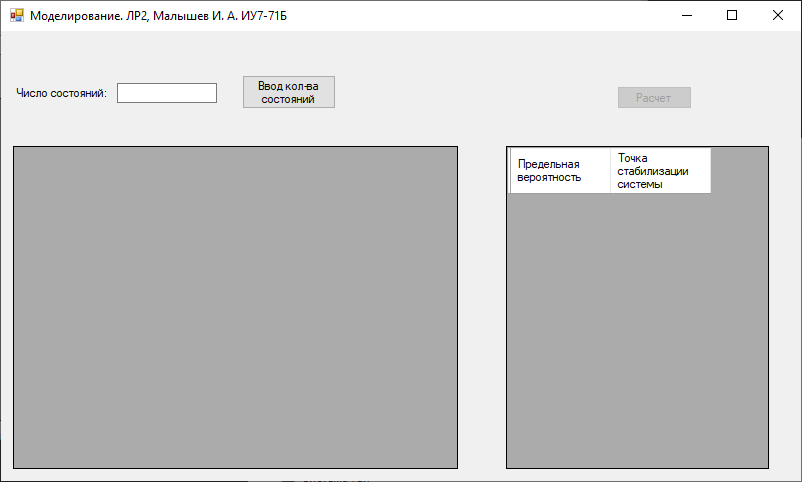
\includegraphics[scale=0.6]{imgs/ui1.png}
	\end{center}
	\caption{Пользовательский интерфейс программы до ввода количества состояний.}
	\label{img:ui1}
\end{figure}

\begin{figure}[H]
	\begin{center}
		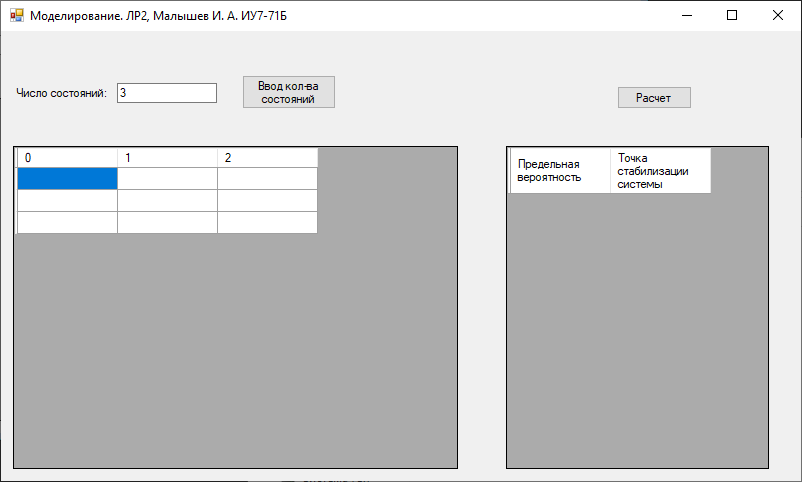
\includegraphics[scale=0.6]{imgs/ui2.png}
	\end{center}
	\caption{Пользовательский интерфейс программы до ввода интенсивностей.}
	\label{img:ui2}
\end{figure}

\subsection{Пример 1}

На рисунках \ref{img:res2}-\ref{img:graph2} представлен пример результатов работы программы с указанными данными.

\begin{figure}[H]
	\begin{center}
		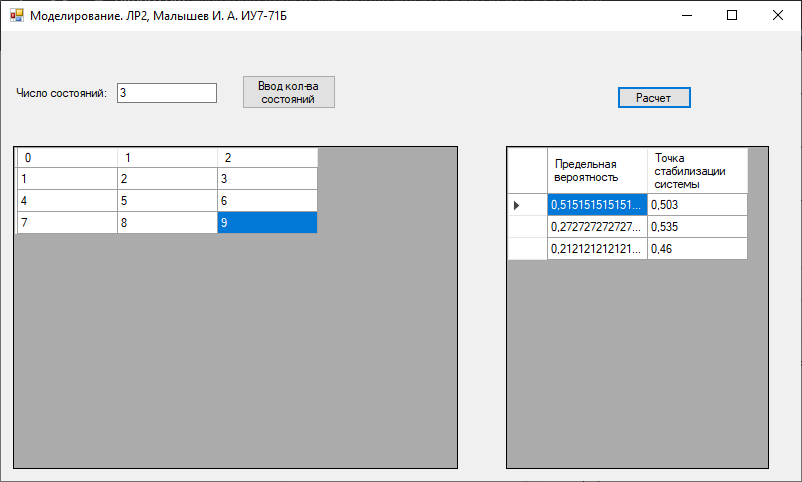
\includegraphics[scale=0.6]{imgs/res2.png}
	\end{center}
	\caption{Исходные данные и результат.}
	\label{img:res2}
\end{figure}

\begin{figure}[H]
	\begin{center}
		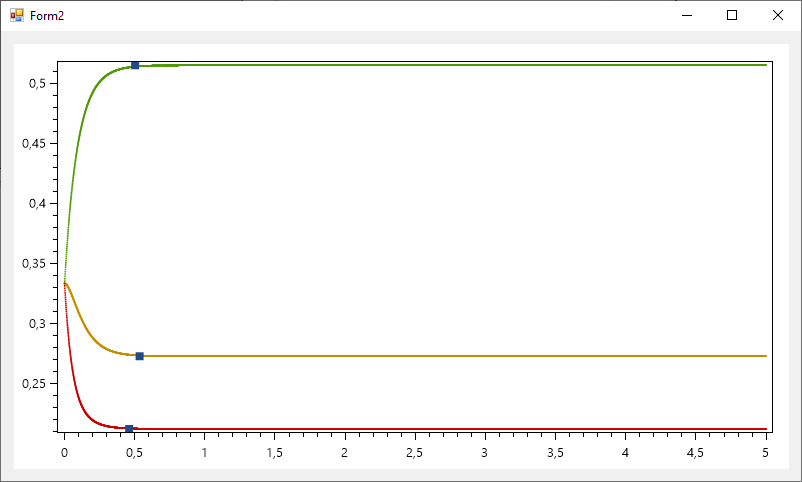
\includegraphics[scale=0.6]{imgs/graph2.png}
	\end{center}
	\caption{График вероятностей с точками стабилизации.}
	\label{img:graph2}
\end{figure}

\subsection{Пример 2}

На рисунках \ref{img:res1}-\ref{img:graph1} представлен пример результатов работы программы с указанными данными.

\begin{figure}[H]
	\begin{center}
		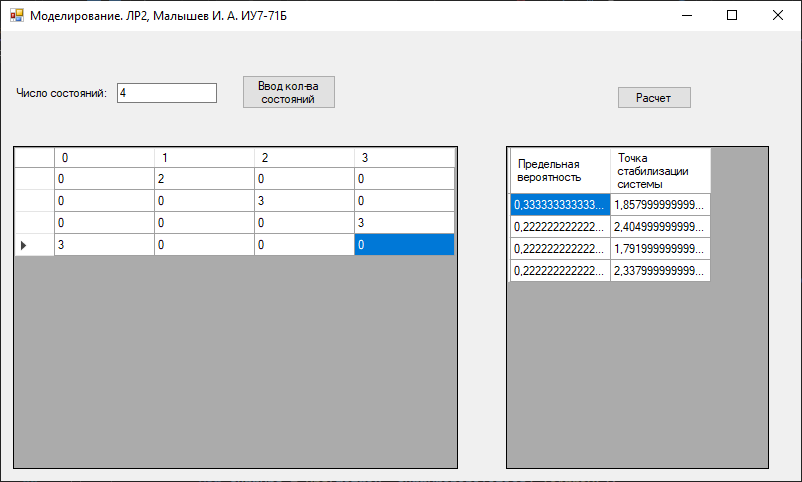
\includegraphics[scale=0.6]{imgs/res1.png}
	\end{center}
	\caption{Исходные данные и результат.}
	\label{img:res1}
\end{figure}

\begin{figure}[H]
	\begin{center}
		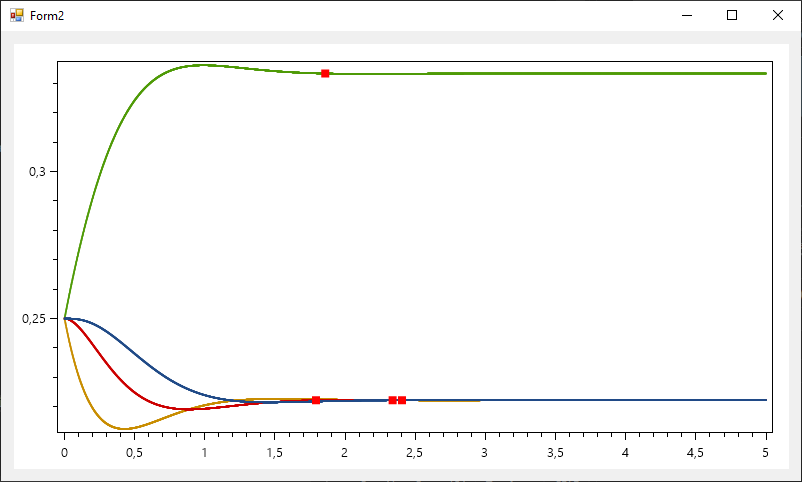
\includegraphics[scale=0.6]{imgs/graph1.png}
	\end{center}
	\caption{График вероятностей с точками стабилизации.}
	\label{img:graph1}
\end{figure}

\end{document}